\section{راهکار پیشنهادی}

\begin{frame}{راهکار پیشنهادی}
	\begin{itemize}\RTList
		\فقره ایجاد مدلی برای ارزیابی سیستم توزیع‌بار (لایه همنوازی).
		
		\فقره پیاده سازی و ارزیابی الگوریتم‌های ارائه شده در مدل تهیه‌شده.
		
		\فقره ایجاد یک الگوریتم توزیع‌بار جدید با توجه به اطلاعات بدست آمده.
	\end{itemize}
\end{frame}

\begin{frame}{جزئیات مهم مدل}
	\begin{itemize}\RTList
		\فقره تعداد محیط‌های اجرا پیوسته تغییر می‌کند.
		
		\فقره سرد و یا گرم بودن محیط اجرا در کارایی تاثیر دارد.
		
		\فقره قرار دادن زنجیره بر روی یک ماشین باعث افزایش کارایی می‌شود.

		\فقره نسبت تعداد محیط‌های در حال اجرا به توان سخت‌افزاری ماشین در کارایی تاثیر گذار است.
	\end{itemize}
\end{frame}

\begin{frame}{جزئیات مهم مدل}
	\begin{figure}[!h]
		\centering
		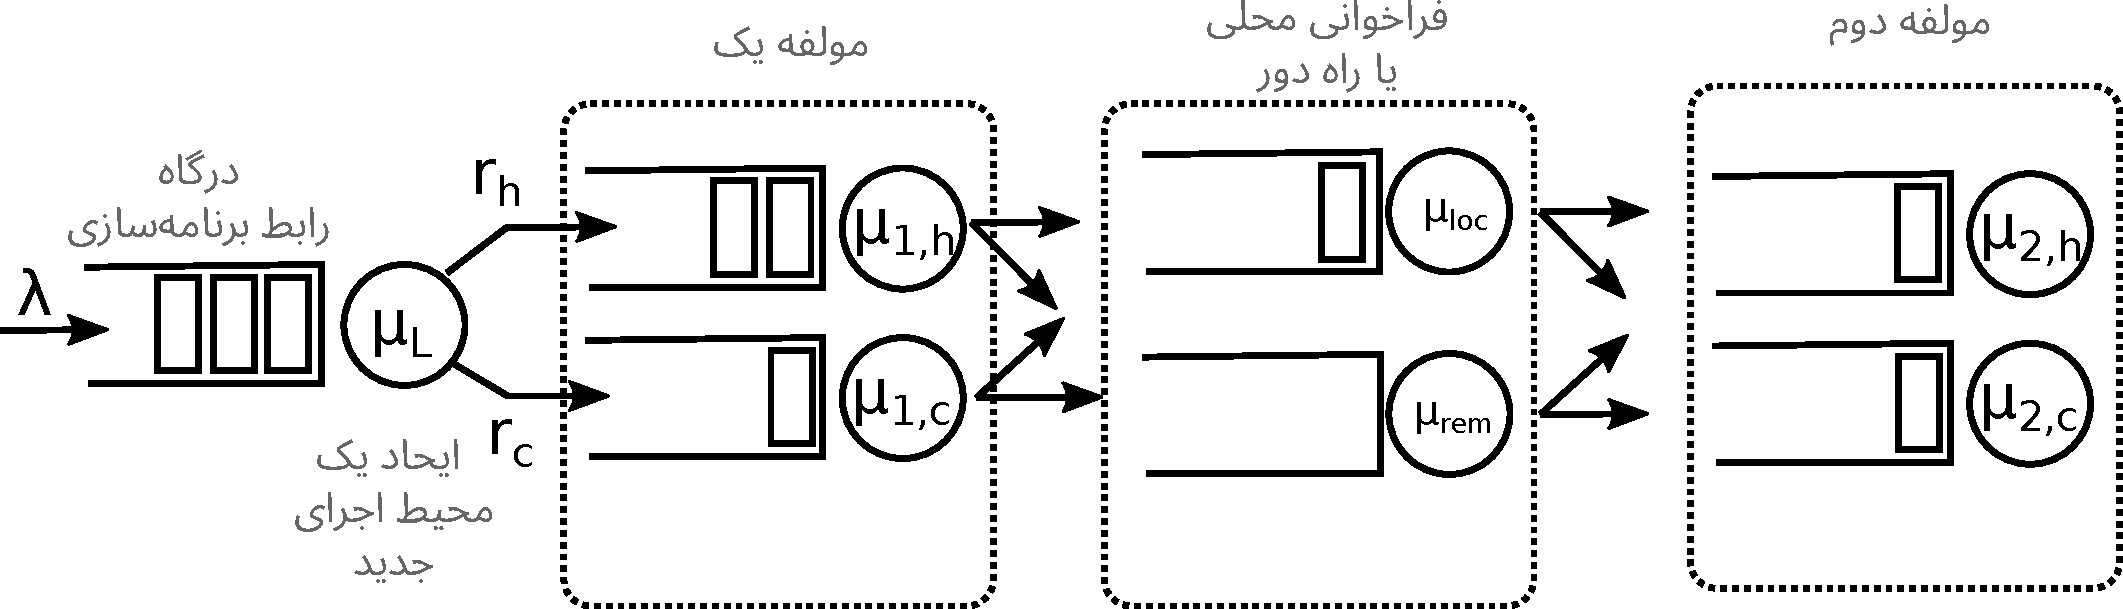
\includegraphics[width=0.8\linewidth]{res/queuing_model.pdf}
		\شرح{مدل پیشنهادی برای سکو پردازش بدون‌میزبان}
		\برچسب{مدلپیشنهادی}
	\end{figure}
\end{frame}

\begin{frame}{جزئیات مهم مدل}
	\begin{table}
		\centering
		\begin{tabular}{|l|r|}
			\hline
			نماد & توضیح 
			\\ \hline
			$m_{i,j}$ &
			تعداد محیط اجرا گرم برای مولفه $f_i$ برای سرور $j$
			\\ \hline
			$select(j)$ &
			احتمال انتخاب خدمت‌گزار $j$ (وابسته به وضعیت سیستم و الگوریتم انتخابی)
			\\ \hline
			 $q_{i,h,j}$  &
			 تعداد درخواست‌های درون صف پردازش گرم
 			\\ \hline
 			$r_{i,h,j}$ &
 			احتمال ورود به صف گرم (وابسته به $m_{i,j}$)
 			\\ \hline
			$r_{i,c,j}$ &
 			احتمال ورود به صف سرد ($1-m_{i,j}$)
 			\\ \hline
 			$\mu_L$ &
 			نرخ سرویس‌دهی توزیع‌کننده بار
 			\\ \hline
 			$\mu_{i,c}$ &
 			نرخ سرویس‌دهی محیط اجرای مولفه $f_i$ در حالت سرد.
 			\\ \hline
			$\mu_{loc}$ &
 			نرخ سرویس‌دهی درخواست‌های محلی.
 			\\ \hline
			$\mu_{rem}$ &
			نرخ سرویس‌دهی درخواست‌های راه‌دور.
			\\ \hline 			
		\end{tabular}
	\end{table}
\end{frame}

\begin{frame}{اعتبار سنجی}
	\begin{itemize}\RTList
	\فقره برای ارزیابی درستی مدل ارائه شده، نتایج آن را با مشاهدات عملی مقایسه می‌شود.
	\فقره برای این منظور می‌توان از ردپاهای ارائه شده در \مرجع{shahrad2020serverless}،
	که مربوط به سکوی پردازش بدون‌میزبان آژور برای شرکت مایکروسافت است،
	استفاده کرد و یا به جمع‌آوری ردپا پرداخت.
	\end{itemize}
\end{frame}

%\begin{figure}[!h]
%	\centering
%	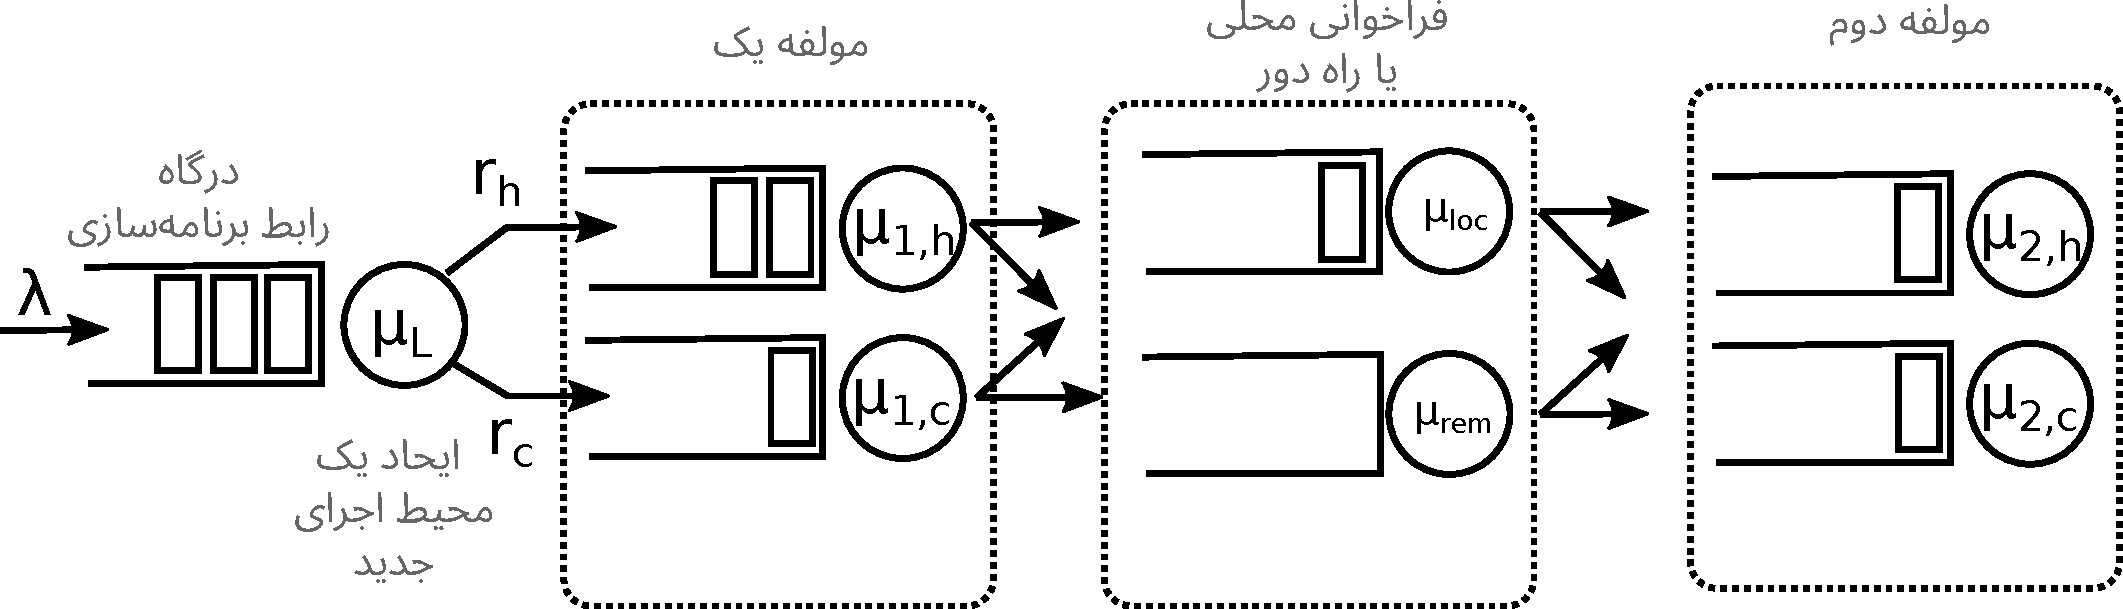
\includegraphics[width=0.9\linewidth]{res/queuing_model.pdf}
%	\شرح{مدل پیشنهادی برای سکو پردازش بدون‌میزبان}
%	\برچسب{مدلپیشنهادی}
%\end{figure}
%
%\begin{figure}[!h]
%	\centering
%	\begin{tikzpicture}
%		\node[state](p0){گرم : 0};
%		\node[state, right=of p0](p1){گرم : 1};
%		\node[state, right=of p1](p2){گرم : 2};
%		\node[right=of p2](p3){$\cdots$};
%		\node[state, right=of p3](pc){$\cpu$};
%		\draw[every loop, ->, line width = 1pt]
%		(p0) edge[bend left] node{} (p1)
%		(p1) edge[bend left] node{} (p0)
%		(p1) edge[bend left] node{} (p2)
%		(p2) edge[bend left] node{} (p1)
%		(p2) edge[bend left] node{} (p3)
%		(p3) edge[bend left] node{} (p2)
%		(p3) edge[bend left] node{} (pc)
%		(pc) edge[bend left] node{} (p3)
%		(pc) edge[loop above] node{\rl{صرف نظر}} (pc)
%		;
%	\end{tikzpicture}
%\شرح{تعداد محیط‌های گرم موجود بر روی خدمت‌گزار}
%\برچسب{مارکوفگرم}
%\end{figure}
%
%در این پروژه برای مقایسه الگوریتم‌های متفاوت توزیع‌بار،
%لایه همنوازی سکوی پردازش بدون‌میزبان مدل‌سازی می‌شود. 
%انتظار می‌رود که با توجه مدل‌ ارائه شده
%بتوان الگوریتم‌های توزیع بار مختلف را ارزیابی کرد. به همین جهت
%مدل ارائه شده باید بتواند وضعیت محیط اجرا را با جزئیات کافی در بر
%بگیرد. مدل ساختار مفهومی ارائه شده در بخش \رجوع{ساختارمولفه} جزئیات
%اولیه لازم مانند سرد یا گرم بودن محیط اجرا را شامل می‌شود. با تبدیل
%این مدل به یک مدل ارزیابی کارایی و اضافه کردن مواردی مانند اجرای زنجیره
%بر روی خدمت‌گزار محلی یا راه دور، در تلاش برای ایجاد یک مدل جامع با جزئیات لازم هستیم.
%
%یک مدل پیشنهادی به صورتی که در ادامه آمده است، ارائه می شود.
%برای هر زنجیره اجرا مراحلی مانند شکل \رجوع{مدلپیشنهادی} در نظر گرفته می‌شود.
%به ازای هر خدمت‌گزار و به ازای هر مولفه فعال در آن خدمت‌گزار دو صف در نظر گرفته می‌شود.
%یک صف برای حالت سرد و یک صف برای حالت گرم. مولفه‌های مربوط به یک خدمت‌گزار به دو صف
%متصل می‌شود. این دو صف نشان می‌دهد که آیا پیام به خدمت‌گزار دیگری ارسال می‌شود و یا اینکه
%در ماشین محلی پردازش می‌شود. اگر $|F|$ تعداد مولفه‌ها باشد و $N$ تعداد خدمت‌گزار‌ها باشد
%و در هر خدمت‌گزار تمام مولفه‌ها فعال باشد آنگاه تعداد صف‌های پردازش (سرد و گرم) عبارت
%است از $|F| \times N \times 2$  و تعداد صف‌های فراخوانی (محلی یا راه دور)
%برابر با $N \times 2$ است.
%
%شکل \رجوع{مدلپیشنهادی} مدلی برای یک زنجیره اجرا دو مولفه‌ای با یک خدمت‌گزار است.
%پیام‌ها پس از بررسی در توزیع‌کننده بار به یک خدمت‌گزار ارسال می‌شود.
%بر روی خدمت‌گزار $j$ تعداد $m_{i,j}$ محیط اجرا گرم برای مولفه $i$ وجود دارد.
%تعداد محیط‌های اجرای گرم از زنجیره شکل \رجوع{مارکوفگرم} پیروی می‌کند.
%
%با احتمال $select(j)$ توزیع‌کننده بار خدمت‌گزار $j$ را انتخاب می‌‌کند.
%با احتمال $r_h$ در خواست در یک محیط اجرای گرم پردازش می‌شود
%در غیر اینصورت درخواست منجر به ایجاد یک محیط اجرای جدید می‌شود.
%مقدار $r_h$ وابسته به $m_{i,j}$، تعداد درخواست‌های درون صف $q_{i,h,j}$ و
%سیاست توزیع‌بار است. مقدار $r_c$ برابر با $1 - r_h$ است.
%
%مقادیر 
%$\mu_L$،
%$\mu_{i,c}$،
%$\mu_{loc}$
%و $\mu_{rem}$ ثابت هستند.
%نرخ سرویس دهی محیط گرم به صورت زیر محاسبه  می‌شود.
%
%\begin{equation}
%	\mu_{i,h,j} = m_{i,j} \times \mu_{h}(f_i)
%\end{equation}
%
%طول صف برای حالت گرم به صورت زیر محاسبه می‌شود و در آن $k_{hot}$ یک پارامتر 
%ثابت سیستم است که حداکثر تعداد رخداد‌ منتظر در یک صف محیط اجرا را مشخص می‌کند.
%
%\begin{equation}
%	k_{i,hot} = m_{i,j} \times k_{hot}
%\end{equation}
%
%
%در این مدل هر زنجیره اجرا، بار کاری منحصر به فردی دارد که به صورت $\lambda_i$
%در نظر گرفته می‌شود.
%
%محاسبه شاخص‌های کارایی به صورت تحلیلی از روی مدل ارائه شده دست بررسی است.
%از طرفی این مدل می‌تواند چارچوبی برای انجام شبیه‌سازی باشد.
%
%برای ارزیابی درستی مدل ارائه شده، نتایج آن را با مشاهدات عملی مقایسه می‌کنیم.
%برای این منظور می‌توان از ردپاهای ارائه شده در \مرجع{shahrad2020serverless}،
%که مربوط به سکوی پردازش بدون‌میزبان آژور\زیرل{Azure} برای شرکت مایکروسافت\زیرل{Microsoft} است،
%استفاده کرد و یا به جمع‌آوری ردپا پرداخت.
%
%پس از صحت سنجی مدل می‌توان با پیاده سازی سیاست‌های مختلف توزیع‌بار،
%که با تنظیم احتمالات ارسال رخداد به خدمت‌گزار‌های مختلف صورت می‌گیرد،
%آن‌ها را ارزیابی کرد. درنهایت از نتایج بدست آمده می‌توان برای
%ایجاد یک الگوریتم توزیع‌بار جدید استفاده کرد.
%
%پس از بدست آمدن مدلی برای ارزیابی روش‌های مختلف توزیع‌بار،
%این فرصت فراهم می‌شود تا از روش‌های یادگیری ماشین اقدام به ایجاد
%یک سیستم توزیع‌بار جدید شود. مدل بدست آمده می‌تواند به عنوان معیار بازخورد
%به الگوریتم‌هایی مانند یادگیری تقویتی استفاده شود.